\section{Il gioco della vita}
\label{sec:the_game_of_life}
Il gioco della vita \`e un automa cellulare\footnote{Un automa cellulare non \`e altro che una griglia regolare di celle in cui ogni cella pu\`o avere un numero finito di stati (per esempio ``acceso'' e ``spento''). Uno stato iniziale (t=0) \`e stabilito assegnando uno stato ad ogni cella. Una \textbf{nuova generazione} \`e creata (avanzando t di 1) in accordo ad alcune regole che determinano un nuovo stato per ogni cella a partire dallo stato precedente.} ideato dal matematico inglese John Horton Conway nel 1970. Il ``gioco'' non ha giocatori, nel senso che la sua evoluzione dipende da uno stato iniziale e non ha bisogno di interazioni umane, lo stato successivo \`e interamente calcolato a partire da quello precedente.

\subsection{Regole}
\label{sec:rules}
Il gioco della vita pu\`o essere ridotto ad alcune semplici regole:
\begin{itemize}
  \item Si svolge su una griglia di caselle quadrate (\textbf{celle}) questa griglia \`e detta \textbf{mondo}.
  \item Il mondo gira attorno: la colonna sul lato sinistro \`e considerata successiva a quella destra (e viceversa), la riga superiore \`e considerata successiva a quella inferiore (e viceversa).
  \item Ogni cella ha 8 \textbf{vicini}, che sono le celle ad essa adiacenti in verticale, orizzontale e diagonale.
  \item Ogni cella pu\`o trovarsi in uno tra due stati: \textbf{viva} o \textbf{morta}.
  \item Gli stati di tutte le celle ad un dato istante sono utilizzati per calcolare lo stato successivo in accordo con le seguenti regole:
  \begin{itemize}
    \item Ogni cella viva con meno di due vicini vivi muore, per isolamento.
    \item Ogni cella viva con pi\`u di tre vicini vivi muore, per sovraffollamento.
    \item Ogni cella viva con due o tre vicini vivi sopravvive (resta viva).
    \item Ogni cella morta con esattamente tre vicini vivi nasce (diventa una cella viva).
  \end{itemize}
  \item Tutte le celle del mondo vengono cos\`i aggiornate simultaneamente nel passaggio da un istante a quello successivo: passa cos\`i una \textbf{generazione}.
\end{itemize}
Di seguito \`e riportato un esempio del gioco della vita in una griglia 10x10 (il mondo) dove si pu\`o vedere come evolgono gli stati delle celle in tre generazioni successive. Le celle vive sono rappresentate con quadrati neri, quelle morte con quadrati bianchi.
\begin{center}
\begin{tabular}{ccc}
  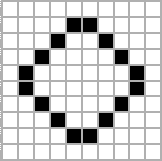
\includegraphics[width=3cm]{octagon2-1.png} &
  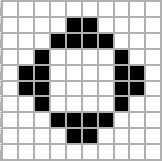
\includegraphics[width=3cm]{octagon2-2.png} &
  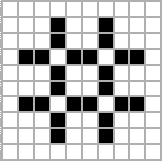
\includegraphics[width=3cm]{octagon2-3.png} \\
  \emph{t = 0} &
  \emph{t = 1} &
  \emph{t = 2} \\
\end{tabular}
\end{center}


\subsection{Algoritmi}
\label{sec:algorithms}
Per rappresentare e simulare il gioco della vita sono stati studiati diversi algoritmi e strutture dati, soprattutto con lo scopo di ottimizzare i calcoli delle generazioni successive (quindi per velocizzare computazioni di molte generazioni) o per rappresentarlo nel modo pi\`u completo possibile, ad esempio permettendo un mondo ``infinitamente'' grande.

La prima e pi\`u semplice rappresentazione \`e attraverso una matrice (o un array bidimensionale) in cui ogni oggetto della matrice rappresenta una cella del gioco della vita, e pu\`o prendere valore 1 o 0 per rappresentare le celle rispettivamente vive o morte. In questo caso l'algoritmo per il calcolo della generazione successiva costruisce una nuova matrice di dimensioni identiche alla prima, per ogni cella conta il numero di vicini vivi e in base a tale numero decide il nuovo stato della cella (viva o morta, 1 o 0) nella nuova matrice.

Un'ottimizzazione a questo algoritmo potrebbe tenere conto che se una cella non ha cambiato stato nell'ultima generazione e nessuno dei suoi vicini ha cambiato stato, allora tale cella sicuramente non cambier\`a stato nella nuova generazione; un algoritmo pi\`u furbo pu\`o quindi mantenere traccia delle zone che non hanno subito cambiamenti nell'ultima generazione ed evitare molti conti inutili.

Per il calcolo di grandi quantit\`a di generazioni \`e stato invece studiato un sofisticato algoritmo, l'HashLife, che sfrutta il comportamento ripetitivo di molte configurazioni (patterns) del gioco della vita per evitare di dover eseguire sempre gli stessi calcoli, in questo modo si riescono a calcolare miliardi di miliardi di generazioni in pochi secondi (``saltando'' per\`o dei passi intermedi).

Se si vuole invece rappresentare un mondo infinito, senza confini, allora si deve cambiare struttura dati, non pi\`u una matrice ma un array di coordinate delle celle vive, in questo modo si riuscirebbe a rappresentare un mondo praticamente infinito (limitato solamente dal massimo numero rappresentabile sul calcolatore per le coordinate estreme), ma chiaramente il conto dei vicini vivi si trasformerebbe in una ricerca sul vettore, aumentando la complessit\`a del calcolo di nuove generazioni.

In questo documento si ci vuole per\`o concentrare sul calcolo parallelo e distribuito, percui per rappresentare il gioco della vita viene preso il primo modello, quello pi\`u semplice ed intuituvo, una matrice di 1 e 0. Con questa struttura l'algoritmo per il calcolo della generazione successiva \`e molto semplice e riportato di seguito in pseudo-codice.

Sia \texttt{M1} una matrice di \texttt{R} righe e \texttt{C} colonne che rappresenta uno stato del gioco della vita. Sia \texttt{M2} una matrice delle dimensioni di \texttt{M1}. Allora l'algoritmo \texttt{generazione\_successiva} calcola la generazione successiva rispetto alla matrice \texttt{M1} e mette il risultato nella matrice \texttt{M2}:
\begin{verbatim}
generazione_successiva(M1, R, C, M2) {
  for I from 0 to R do
    for J from 0 to C do
      V := numero_vicini_vivi(M1,I,J);
      if M1[I][J] == 1 then
        if V == 2 or V == 3 then
          M2[I][J] := 1;           // la cella sopravvive
        else 
          M2[I][J] := 0;           // la cella muore
        endif
      else
        if V == 3  then
          M2[I][J] := 1;           // la cella "nasce"
        else
          M2[I][J] := 0;           // la cella rimane morta
        endif
      endif
    endfor
  endfor
}
\end{verbatim}
\label{alg:nextgeneration}
Diremo allora che un'\textbf{iterazione} sulla matrice che rappresenta il gioco della vita \`e l'applicazione dell'algoritmo precedente su di essa, sostituendola infine con la nuova matrice (\texttt{M2}). Compiere \textit{n} iterazioni sulla matrice vorr\`a quindi dire calcolare \textit{n} generazioni.

Su una matrice di \textit{r} righe e \textit{c} colonne l'algoritmo ha costo nell'ordine di $8*r*c$, infatti \`e previsto che siano fatti otto controlli (per il calcolo del numero di vicini vivi) per ogni elemento della matrice; nel caso di matrici quadrate il costo dell'algoritmo \`e quindi esponenziale. Una simulazione del gioco della vita consister\`a nel compiere \textit{n} iterazioni dell'algoritmo, il che \`e ovviamente molto costoso per matrici di grandi dimensioni. Questi tempi possono essere ammortizzati distribuendo il calcolo in parallelo.
